\section{Settings for using COMPAS}
\label{sec:appA}
To generate a binary systems, COMPAS requires the following parameters from the user as discussed earlier,
\begin{itemize}
    \item mass of primary star $(\mone{ZAMS})$,
    \item mass of secondary star $(\mtwo{ZAMS})$,
    \item semi-major axis of the orbit $(\semaxis{ZAMS})$,
    \item random seed $(\o)$
    \item remnant mass prescription,
    \item eccentricity of the orbit $(\ecc{ZAMS})$, and
    \item metallicity of the stars $\left(Z\right)$.
\end{itemize}

We've discussed the first four parameters in the main text, here we will discuss the selection of eccentricity and metallicity values.

\begin{center}%
    \section*{Eccentricity}
    \label{sec:eccentricity}
\end{center}%

In order to evaluate whether the initial eccentricity affects GW emission at the end stages of the DCO, we generate two identical data sets.
For the primary data set, we chose the eccentricity value to be varied between 0 and 1.
For the selection of eccentricity, the power law and gamma distribution were also considered.\@\\

\subsection{Power law distribution}
\label{subsec:power-law-distribution}
The random values for metallicity were generated using the power law distribution given below,
\begin{equation}
    f(x, a) = ax^{(a-1)}
    \label{eq:powerlaw_distribution}
\end{equation}
where $a$ is the index of the power law distribution.\footnote{\url{https://docs.scipy.org/doc/scipy/reference/generated/scipy.stats.powerlaw.html}}
Figure~\ref{fig:pl_distribution} shows the plot for the probability density function (PDF) of the power law with $a \in [1, 2]$.
Although the distribution can produce higher values, it does not suppress the lower values so this distribution was discarded.

\subsection{Gamma distribution}
\label{subsec:gamma-distribution}
For the probability density function for gamma distribution,\footnote{\url{https://docs.scipy.org/doc/scipy/reference/generated/scipy.stats.gamma.html}} we use the following form,
\begin{equation}
    f(x, a) = \frac{x^{a-1}\exp(-x)}{\Gamma(a)}
    \label{eq:gamma_distribution}
\end{equation}
for $x\geq 0$ and $a > 0$.
Here, $a$ is the shape factor, and $\Gamma$ is the gamma function, such that $\Gamma(a) = (a-1)!$.
Similar to the power law distribution, the gamma distribution (see, figure~\ref{fig:gamma_distribution}) was not a good selection for the values of metallicity that were required for this study.

\subsection{Beta distribution}
\label{subsec:beta-distribution}

For the beta distribution, we use the following form,
\begin{equation}
    f(x, a, b) = \frac{\Gamma(a+b)x^{a-1}(1-x)^{b-1}}{\Gamma(a)\Gamma(b)}
    \label{eq:beta_distribution}
\end{equation}
For $0 \leq x \leq 1, a > 0, b > 0$ and $\Gamma$ is the gamma function.\footnote{\url{https://docs.scipy.org/doc/scipy/reference/generated/scipy.stats.beta.html}}

Figure~\ref{fig:beta1} shows the beta distribution with a fixed $\beta=80$.
Similarly, figure~\ref{fig:beta2} shows the beta distribution with a fixed $\alpha=5$.
For our case, we selected $\text{Beta}(5, 80)$ as our distribution of choice for metallicity and generated $10^7$ values between the COMPAS limits $10^{-4} < z < 0.03$.

\begin{minipage}[l]{0.48\textwidth}
    \centering
    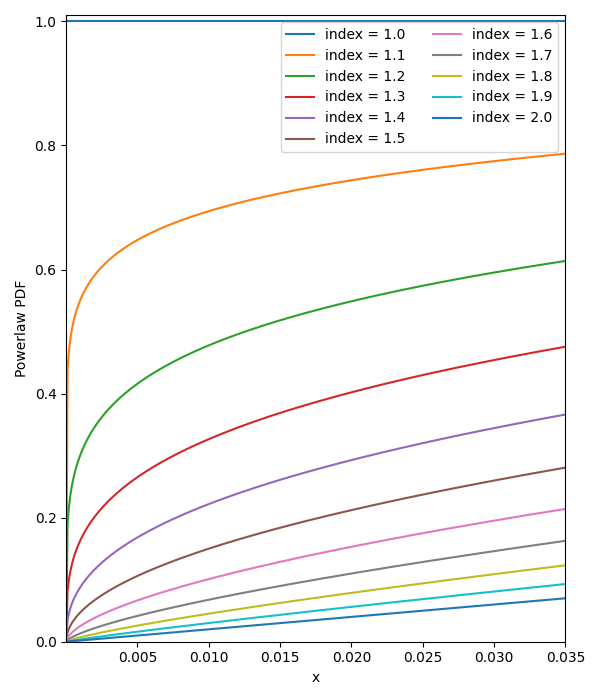
\includegraphics[width=\textwidth]{images/powerlaw}
    \captionof{figure}{Power-law distribution}
    \label{fig:pl_distribution}
\end{minipage}
\hfill
\begin{minipage}[c]{0.48\textwidth}
    \centering
    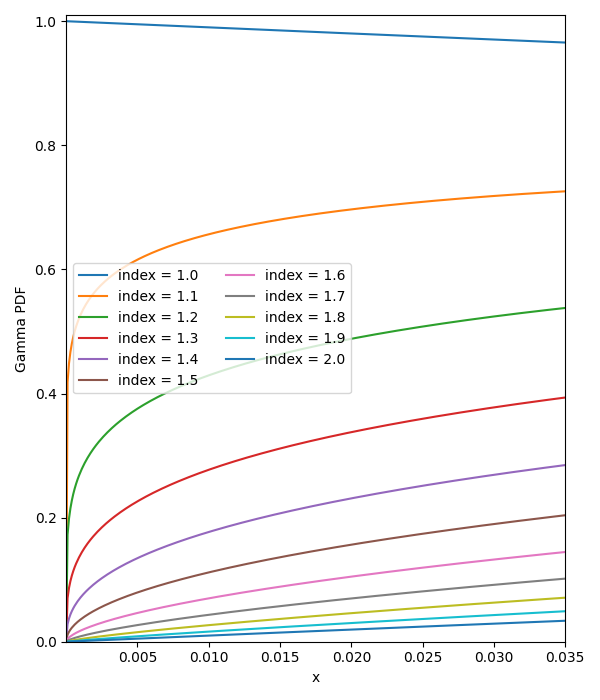
\includegraphics[width=\textwidth]{images/gamma}
    \captionof{figure}{Gamma distribution}
    \label{fig:gamma_distribution}
\end{minipage}

\hfill

\begin{minipage}[l]{0.48\textwidth}
    \centering
    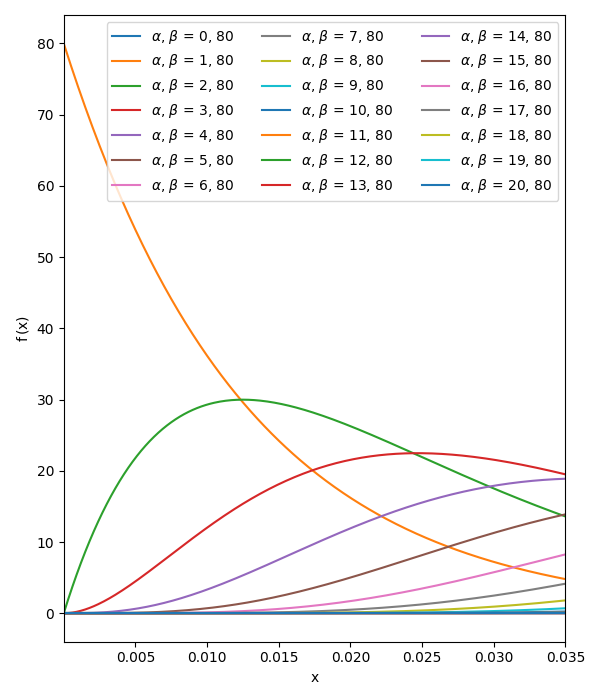
\includegraphics[width=\textwidth]{images/beta1}
    \captionof{figure}{Beta distribution with varying $\alpha$ and fixed $\beta$ parameter.}
    \label{fig:beta1}
\end{minipage}
\hfill
\begin{minipage}[c]{0.48\textwidth}
    \centering
    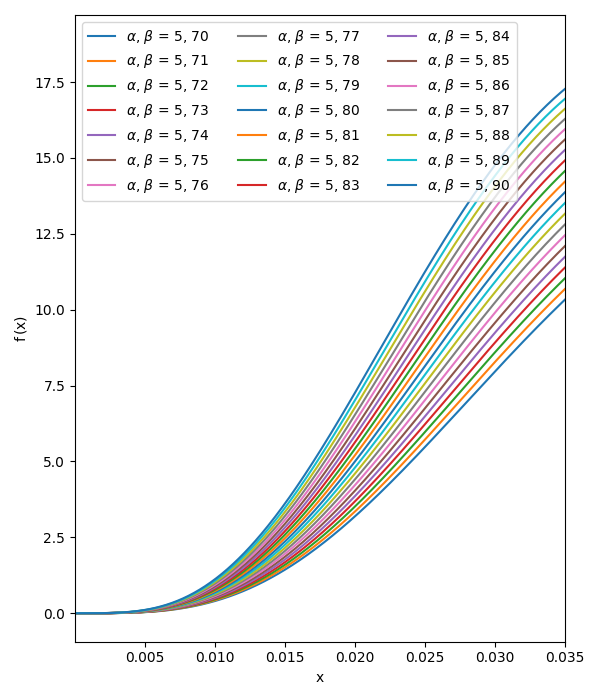
\includegraphics[width=\textwidth]{images/beta2}
    \captionof{figure}{Beta distribution with fixed $\alpha$ and varying $\beta$ parameter.}
    \label{fig:beta2}
\end{minipage}

%The same value for metallicity was used for both stars as different metallicity scenario is highly unlikely.

%\begin{figure}[!ht]%
%    \centering
%    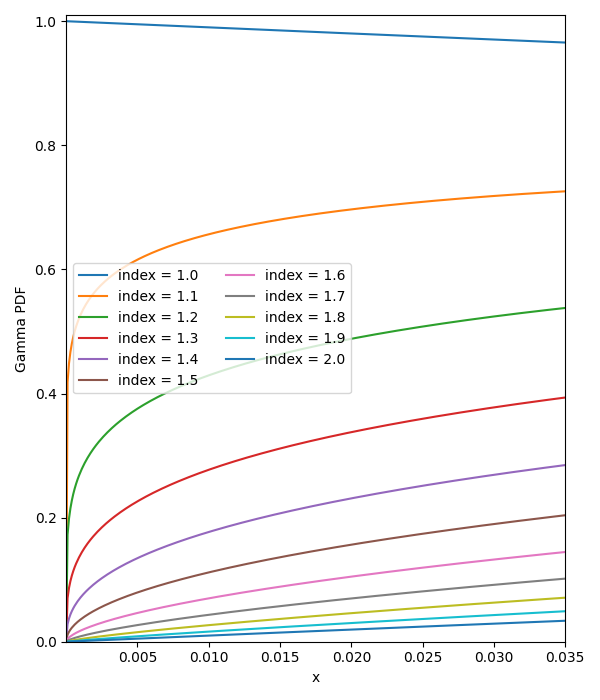
\includegraphics[width=\linewidth]{images/gamma}
%    \caption{Gamma distribution with $1 \leq a \leq 2$.}
%    \label{fig:gamma_distribution}
%\end{figure}%
%\begin{figure}[!ht]%
%    \centering
%    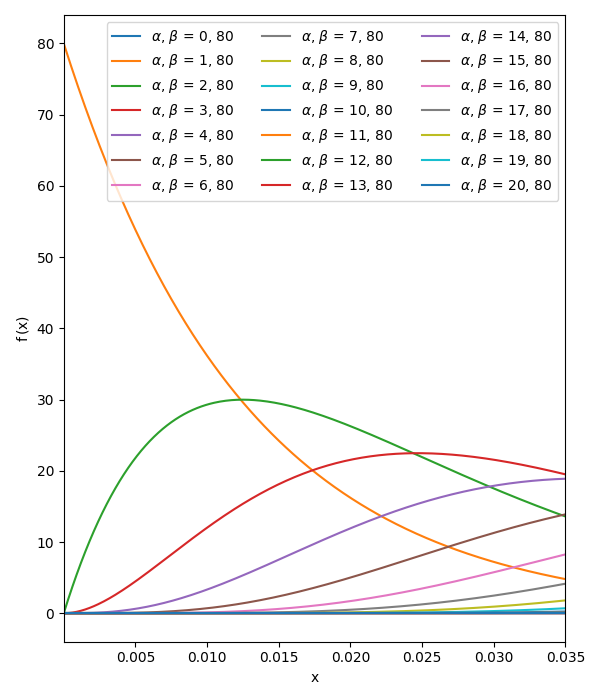
\includegraphics[width=\linewidth]{images/beta1}
%    \caption{Beta distribution with varying $\alpha$ and fixed $\beta$ parameter.}
%    \label{fig:beta1}
%\end{figure}%
%\begin{figure}[!ht]%
%    \centering
%    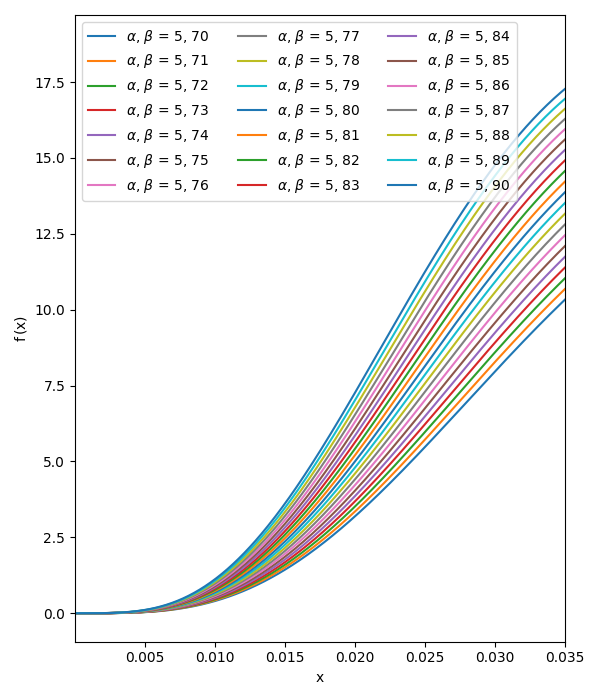
\includegraphics[width=\linewidth]{images/beta2}
%    \caption{Beta distribution with fixed $\alpha$ and varying $\beta$ parameters.}
%    \label{fig:beta2}
%\end{figure}%

\begin{center}
    \section*{Metallicity}
    \label{sec:metallicity}
\end{center}
One of the major challenges in generation of the stellar binaries for this study was the selection of a distribution which will result in stars at the higher end of COMPAS metallicity boundary, $z = 0.03$.
A power-law, gamma, and beta distributions were selected to try and simulate the required metallicity distribution.
In the following section, we discuss the selected distributions briefly,
\newpage\cleardoublepage